\documentclass[10pt,letterpaper]{article}
\usepackage[utf8]{inputenc}
\usepackage[T1]{fontenc}
\usepackage[margin=0.6in]{geometry}
\usepackage{amsmath,amssymb,mathtools,graphicx,booktabs,xcolor,hyperref}
\setlength{\parindent}{0pt}
\setlength{\parskip}{5pt}
\begin{document}

\section*{Block S3 Exercises: RC Charging \& Discharging Transients}

  \textbf{Schedule Window:} Sunday, Oct 18, 5:05--6:05 PM (60 min) ~|~
  \textbf{Total Points:} 40 pts ~|~
  \textbf{Mix:} 2 Calculus Derivations, 1 Two-Stage Switch FR, 1 Aligned Two-Panel Graph



  \textbf{Core Mastery Goals:} (1) Deriving $q(t), v_C(t), i(t)$ by separating variables on the first-order KVL differential equation; (2) Proving by definite integration why a charging resistor dissipates $\frac{1}{2}C\mathcal{E}^2$ regardless of $R$; (3) Applying capacitor voltage continuity $v_C(t_1^+) = v_C(t_1^-)$ and current jump discontinuity across switching events.


\subsection*{01 $\cdot$ First-Order RC Differential Equation \& Separation of Variables \hfill [Ch. 26 $\cdot$ 10 Points $\cdot$ DERIVE]}

An ideal battery of EMF $\mathcal{E} = V_0$ is connected in series with a resistor $R$ and an initially uncharged capacitor $C$ ($q(0) = 0$) as shown in the Spec v2 circuit below, where the switch closes at $t = 0$.

\begin{center}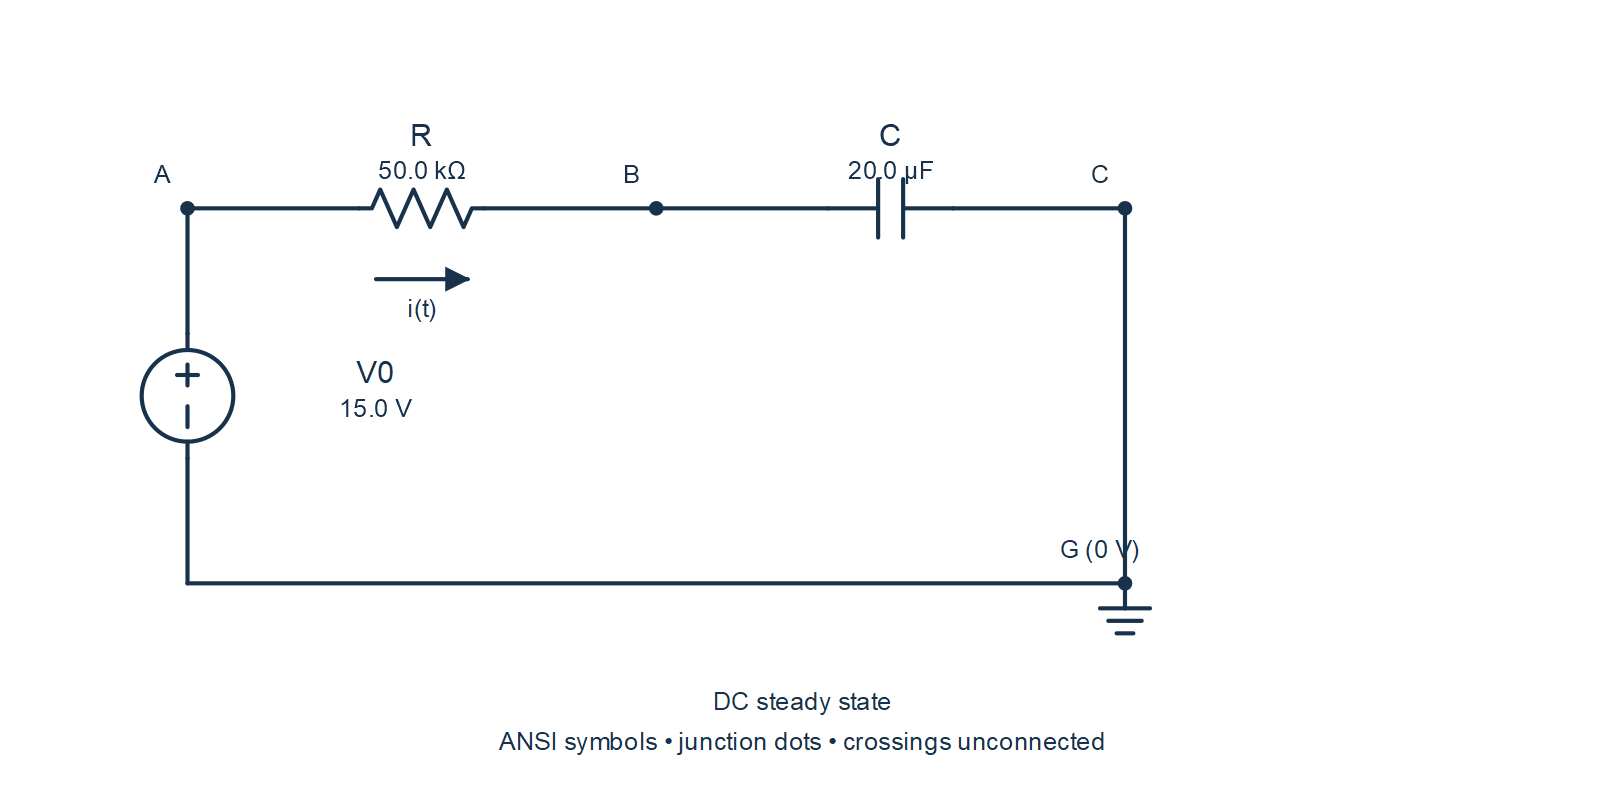
\includegraphics[width=0.82\linewidth]{day1_assets/s3-q1-rc-circuit.png}\end{center}

\begin{enumerate}
  \item \textbf{Charging Differential Equation \& Separation of Variables [6 points]:}
    \begin{enumerate}
      \item Apply Kirchhoff's loop rule around the series circuit for $t \ge 0$ and substitute $i(t) = \dfrac{dq}{dt}$ to write the first-order linear differential equation for $q(t)$. \textbf{[2 pts]}
      \item Separate variables so that all $q$-dependent terms are on the left and all $t$-dependent terms are on the right, and integrate explicitly from $q(0) = 0$ at $t' = 0$ to $q(t)$ at $t' = t$:
      $$\int_{0}^{q(t)} \frac{dq'}{C\mathcal{E} - q'} = \int_{0}^{t} \frac{dt'}{RC}.$$
      Solve for $q(t)$, $v_C(t) = \frac{q(t)}{C}$, and $i(t) = \frac{dq}{dt}$, identifying the capacitive time constant $\tau = RC$. \textbf{[4 pts]}
    \end{enumerate}
  
  \item \textbf{Discharging from Initial Charge $Q_0$ [4 points]:} Suppose the battery is removed and a capacitor carrying initial charge $Q_0 = C V_{\text{init}}$ at $t = 0$ is discharged through resistor $R$. Write the KVL differential equation $\frac{q}{C} + R\frac{dq}{dt} = 0$, separate variables, and integrate from $Q_0$ to $q(t)$ to derive $q(t) = Q_0 e^{-t/RC}$ and $v_C(t) = V_{\text{init}} e^{-t/RC}$.
\end{enumerate}
\vspace{1.2in}


\newpage



\subsection*{02 $\cdot$ Calculus Proof of Energy Conservation \& Half-Energy Dissipation \hfill [Ch. 24, 26 $\cdot$ 10 Points $\cdot$ DERIVE]}

When an initially uncharged capacitor $C$ is charged to final voltage $\mathcal{E}$ through a series resistor $R$ by a constant-EMF battery $\mathcal{E}$, the charging current is $i(t) = \dfrac{\mathcal{E}}{R} e^{-t/(RC)}$ for $0 \le t < \infty$.

\begin{enumerate}
  \item \textbf{Total Charge \& Work Done by the Battery [3 points]:}
    \begin{enumerate}
      \item Integrate the current from $t = 0$ to $t \to \infty$ to verify that the total charge delivered by the battery is $Q_{\text{final}} = \int_0^\infty i(t)\,dt = C\mathcal{E}$.
      \item Using $dW_{\text{batt}} = \mathcal{E}\,dq = \mathcal{E} i(t)\,dt$, show that the total electrical work done by the battery over the entire charging process is:
      $$W_{\text{batt}} = \int_{0}^{\infty} \mathcal{E} i(t)\,dt = C\mathcal{E}^2.$$
    \end{enumerate}
  
  \item \textbf{Joule Heating Integral in the Resistor [5 points]:} The instantaneous rate of thermal energy dissipation in the resistor is $P_R(t) = [i(t)]^2 R$. Set up and evaluate the improper integral:
  $$E_{\text{dissipated}} = \int_{0}^{\infty} [i(t)]^2 R\,dt = \int_{0}^{\infty} \left(\frac{\mathcal{E}}{R} e^{-t/(RC)}\right)^2 R\,dt$$
  to prove that:
  $$E_{\text{dissipated}} = \frac{1}{2} C\mathcal{E}^2.$$
  \item \textbf{Energy Accounting \& Physical Independence from $R$ [2 points]:} Compare $E_{\text{dissipated}}$ with the final electrostatic energy $U_C = \int_0^{C\mathcal{E}} \frac{q}{C}\,dq = \frac{1}{2}C\mathcal{E}^2$ stored in the capacitor, verify $W_{\text{batt}} = U_C + E_{\text{dissipated}}$, and explain mathematically why the resistance $R$ cancels out of $E_{\text{dissipated}}$ (what happens to peak power vs. duration $\tau = RC$ if $R$ is halved?).
\end{enumerate}
\vspace{1.2in}


\newpage



\subsection*{03 $\cdot$ Two-Position Switch RC Transient \& Continuity vs. Jump Analysis \hfill [Ch. 26 $\cdot$ 10 Points $\cdot$ FR + SWITCH]}

In the two-position switch circuit below, $V_0 = 15.0\text{ V}$, $R = 50.0\text{ k}\Omega$, and $C = 20.0\ \mu\text{F}$. The capacitor is initially uncharged ($v_C(0^-) = 0\text{ V}$). At $t = 0$, switch $S$ is thrown to \textbf{Position 1} (connecting the series $RC$ branch to $V_0 = 15.0\text{ V}$) and remains there for $0 \le t < 2.00\text{ s}$. At instant $t_1 = 2.00\text{ s}$, switch $S$ is thrown instantaneously to \textbf{Position 2} (connecting the left end of $R$ directly to ground, $0\text{ V}$, for $t \ge 2.00\text{ s}$). The reference current $i(t) = C\frac{dv_C}{dt}$ is defined flowing rightward into the top plate (Node $B$).

\begin{center}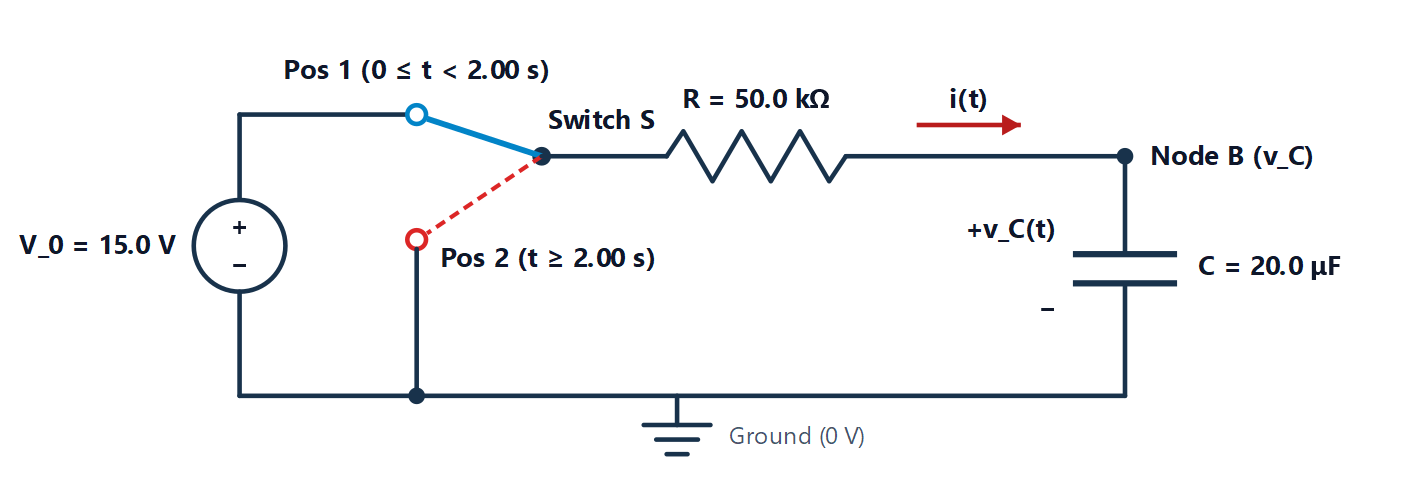
\includegraphics[width=0.82\linewidth]{day1_assets/s3-q3-rc-switch.png}\end{center}

\begin{enumerate}
  \item \textbf{Time Constant \& Initial Charging ($t = 0^+$) [2 points]:} Compute the capacitive time constant $\tau = RC$ (in $\text{s}$), the initial capacitor voltage $v_C(0^+)$, and the initial charging current $i(0^+)$ (in $\mu\text{A}$).
  \item \textbf{State Just Before Switching ($t_1^- = 2.00\text{ s}^-$) [3 points]:} Write the analytical expressions for $v_C(t)$ and $i(t)$ on $0 \le t < 2.00\text{ s}$, and calculate the numerical values of $v_C(2.00\text{ s}^-)$ (in $\text{V}$) and $i(2.00\text{ s}^-)$ (in $\mu\text{A}$).
  \item \textbf{Switching Instant Continuity \& Jump ($t_1^+ = 2.00\text{ s}^+$) [3 points]:}
    \begin{enumerate}
      \item State the value of $v_C(2.00\text{ s}^+)$ immediately after the switch moves to Position 2, and explain physically why $v_C(t)$ cannot jump instantaneously when $R > 0$.
      \item Calculate the signed current $i(2.00\text{ s}^+)$ (in $\mu\text{A}$) immediately after switching to Position 2, and compute the instantaneous jump $\Delta i = i(2.00\text{ s}^+) - i(2.00\text{ s}^-)$.
    \end{enumerate}
  
  \item \textbf{Discharging Regime ($t \ge 2.00\text{ s}$) [2 points]:} Write $v_C(t)$ and $i(t)$ as functions of $(t - 2.00\text{ s})$ for $t \ge 2.00\text{ s}$, and evaluate $v_C(3.50\text{ s})$ (in $\text{V}$) and $i(3.50\text{ s})$ (in $\mu\text{A}$).
\end{enumerate}
\vspace{1.2in}


\newpage



\subsection*{04 $\cdot$ Aligned $v_C(t)$ and $i(t)$ Transient Graphs \& Continuity Cloze \hfill [Ch. 26 $\cdot$ 10 Points $\cdot$ DRAW + CLOZE]}

\subsubsection*{Part A: Draw the Effect --- Aligned Two-Panel Transient Plots [6 points --- DRAW]}
For the two-stage switching circuit of Exercise 03 ($V_0 = 15.0\text{ V}, R = 50.0\text{ k}\Omega, C = 20.0\ \mu\text{F}$, switch thrown from Position 1 to Position 2 at $t_1 = 2.00\text{ s}$):
\begin{enumerate}
  \item \textbf{Graph (i) [3 points]:} On the left grid below, plot the capacitor voltage $v_C(t)$ (\textbf{dependent variable}, vertical axis, in $\text{V}$) vs. time $t$ (\textbf{independent variable}, horizontal axis, in $\text{s}$) from $t = 0$ to $t = 5.00\text{ s}$. Label the coordinates of the cusp peak at $t_1 = 2.00\text{ s}$ and the value at $t = 3.50\text{ s}$ using your results from Exercise 03.
  \item \textbf{Graph (ii) [3 points]:} On the right grid below, plot the signed current $i(t) = C\frac{dv_C}{dt}$ (\textbf{dependent variable}, vertical axis, in $\mu\text{A}$) vs. time $t$ (\textbf{independent variable}, horizontal axis, in $\text{s}$) from $t = 0$ to $t = 5.00\text{ s}$. Mark and label the initial current $i(0^+)$, the pre-switch current $i(2.00\text{ s}^-)$, the post-switch current $i(2.00\text{ s}^+)$, and the value $i(3.50\text{ s})$ calculated in Exercise 03.
\end{enumerate}

\begin{center}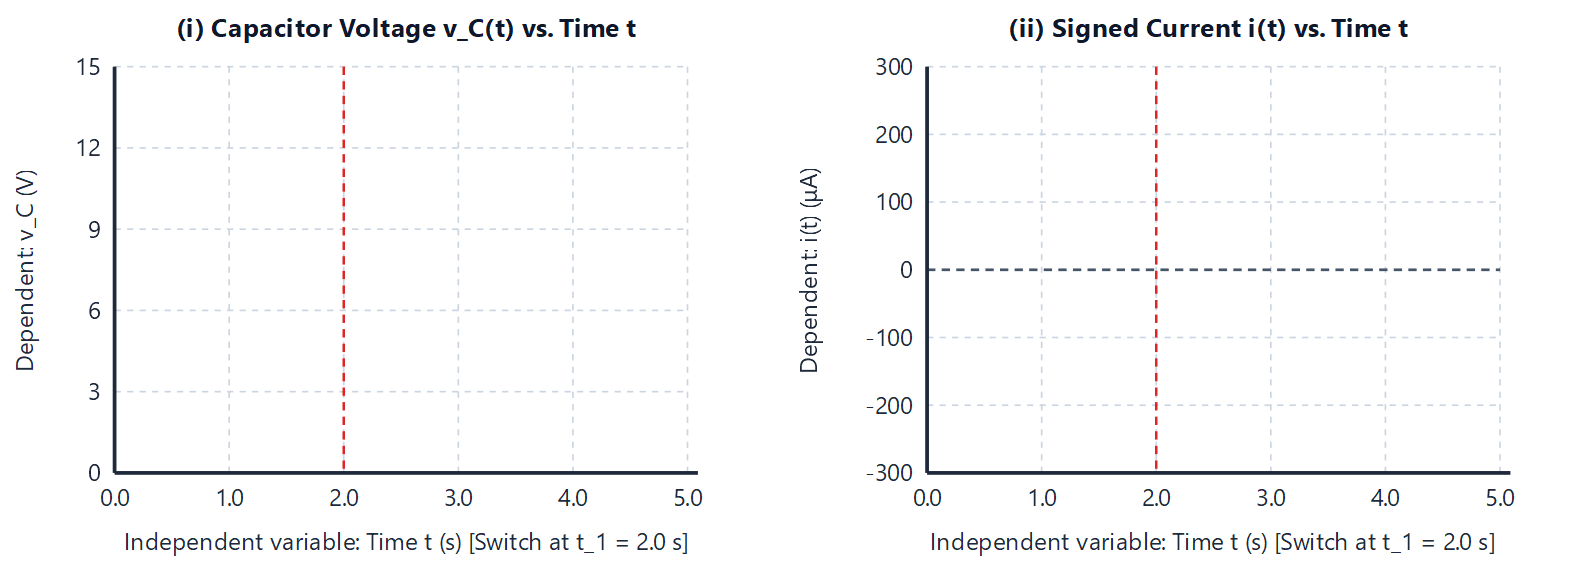
\includegraphics[width=0.82\linewidth]{day1_assets/s3-q4-grid-blank.png}\end{center}

\subsubsection*{Part B: RC Transient \& Continuity Rules Cloze [4 points --- 0.5 point each]}

  \textbf{WORD BANK:} ~
  \texttt{short circuit (wire)} $\cdot$
  \texttt{open circuit} $\cdot$
  \texttt{continuous} $\cdot$
  \texttt{discontinuous} $\cdot$
  \texttt{$63.2\\%$} $\cdot$
  \texttt{$36.8\\%$} $\cdot$
  \texttt{$86.5\\%$} $\cdot$
  \texttt{$\frac{1}{2}C\mathcal{E}^2$} $\cdot$
  \texttt{$C\mathcal{E}^2$} $\cdot$
  \texttt{seconds ($\text{s}$)}


\begin{enumerate}
  \item In SI units, the product $\tau = RC$ has dimensions of $(\text{V/A})\cdot(\text{C/V}) = \text{C/(C/s)}$, which reduces to \underline{\hspace{1.8in}}.
  \item At $t = 0^+$ immediately after a DC source is connected to an uncharged capacitor ($q(0^+)=0 \implies v_C(0^+)=0$), the capacitor momentarily behaves as a \underline{\hspace{1.8in}}.
  \item As $t \to \infty$ in DC steady state, a fully charged capacitor carries zero current ($i(\infty)=0$) and behaves as an \underline{\hspace{1.8in}}.
  \item After one time constant ($t = \tau = RC$) of charging from zero, $v_C(\tau)$ reaches $1 - e^{-1} \approx$ \underline{\hspace{1.8in}} of its final asymptotic voltage $\mathcal{E}$, while the charging current $i(\tau)$ decays to $e^{-1} \approx$ \underline{\hspace{1.8in}} of $i(0^+)$.
  \item Across any finite-current switching instant $t = t_1$, the capacitor voltage $v_C(t)$ must be \underline{\hspace{1.8in}}, whereas the resistor current $i(t)$ is generally \underline{\hspace{1.8in}}.
  \item During complete charging of an uncharged capacitor $C$ from an ideal battery $\mathcal{E}$, the total thermal energy dissipated in the series resistor $R$ is always \underline{\hspace{1.8in}}.
\end{enumerate}

\end{document}
